% Ubah judul dan label berikut sesuai dengan yang diinginkan.
\section{Metode Penelitian}
\label{sec:MetodePenelitian}

Penelitian ini dilaksanakan sesuai sistem berikut dengan implementasinya. Desain sisttem merupakan konsep dari pembuatan dan perancangan infrastruktur yang kemudian diwujudkan dallam bentuk blok diagram alur ang harus dikerjakan. Pada Gambar \ref{fig:BlokMetodologi} menunjukkan bagan umum metodologi sistem.

\begin{figure} [ht]
  \centering
  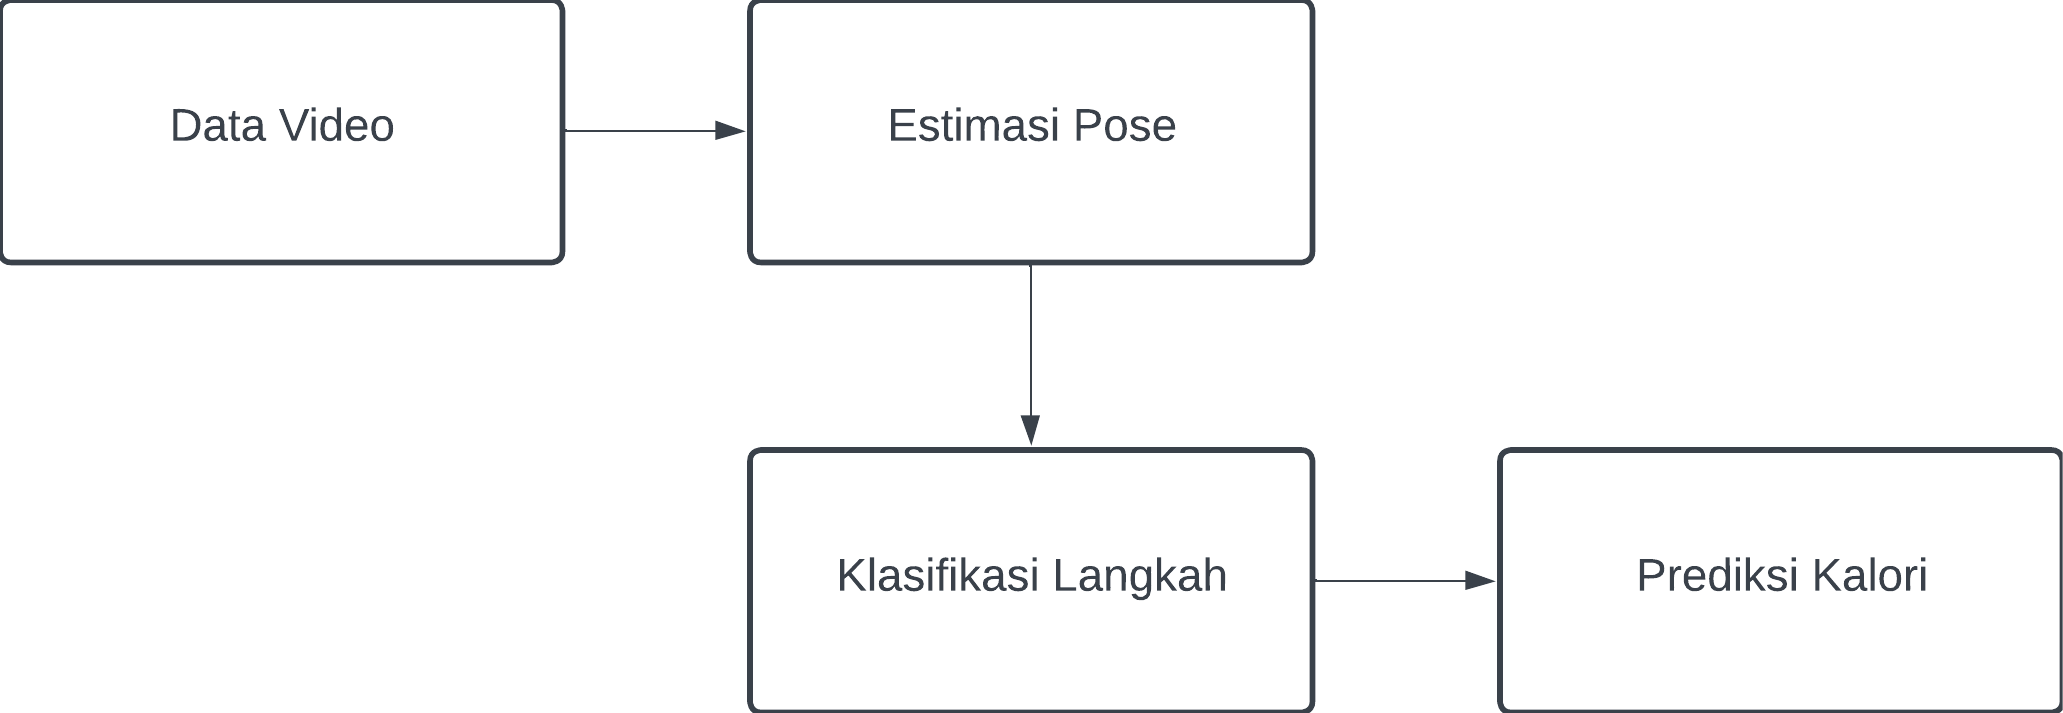
\includegraphics[width=0.4\textwidth]{gambar/blok diagram metodologi4.png}
  \caption{Bagan Umum Metodologi Sistem}
  \label{fig:BlokMetodologi}
\end{figure}

\subsection{Data Video}
\label{subsec:DataVideo}

Pada penelitian ini digunakan data berupa data video yang dilakukan pengambilan data dan diperoleh menggunakan kamera pada \emph{smartphone} atau kamera eksternal yang akan direkam dan disimpan untuk kemudian akan digunakan pada proses yang dilakukan pada perangkat komputer/laptop. Proses pengambilan data dilakukan dengan peraga melakukan aktivitas pada treadmill dengan ditampakkan secara jelas pada tampilan kamera Webcam. Setelah terdapat peraga dan tampak jelas pada tampilan maka data citra akan dilakukan pada tahap selanjutnya untuk dideteksi dan segmentasi pose seperti pada Gambar \ref{fig:DataVideo}. Variasi yang digunakan pada data video yang digunakan berdasarkan variasi kecepatan dan hasil kalori yang terbakar.

\begin{figure} [ht]
  \centering
  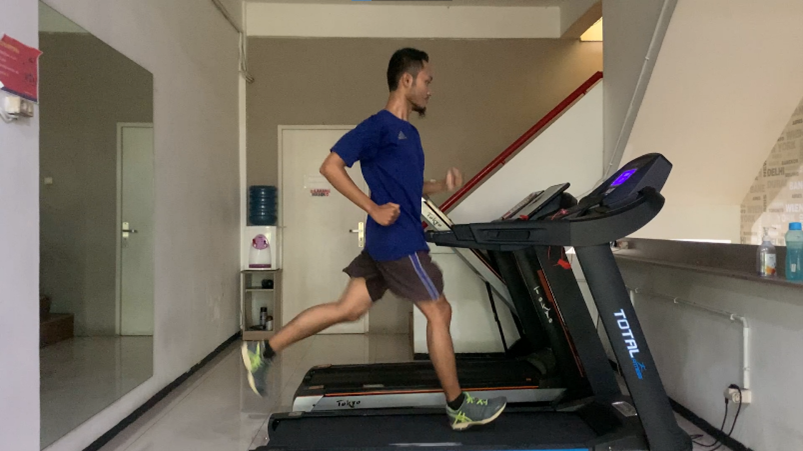
\includegraphics[width=0.4\textwidth]{gambar/pengambilan data.png}
  \caption{Proses Pengambilan Data}
  \label{fig:DataVideo}
\end{figure}

\subsection{Estimasi Pose}
\label{subsec:EstimasiPose}

Estimasi dari hasil citra untuk dapat mengetahui bentuk postur tubuh manusia menggunakan Python dengan \emph{library} OpenCV yaitu MediaPipe. Metode yang digunakan pada MediaPipe menggunakan estimasi pose untuk mendeteksi postur tubuh. Modifikasi dilakukan dengan mengambil kerangka bagian kaki dengan memberikan warna yang berbeda untuk dapat berfokus pada hasil estimasi kaki bagian kiri dan kanan. Segementasi dilakukan dengan cara peraga melakukan aktivitas \emph{jogging} pada treadmill dengan menentukan pose melangkah seperti yang terdapat pada Gambar \ref{fig:EstimasiPose}. Hasil estimasi dari model Mediapipe berupa kerangka yang menyesuaikan bentuk tubuh yang diestimasi dari data video yang dimiliki.

\begin{figure} [ht]
  \centering
  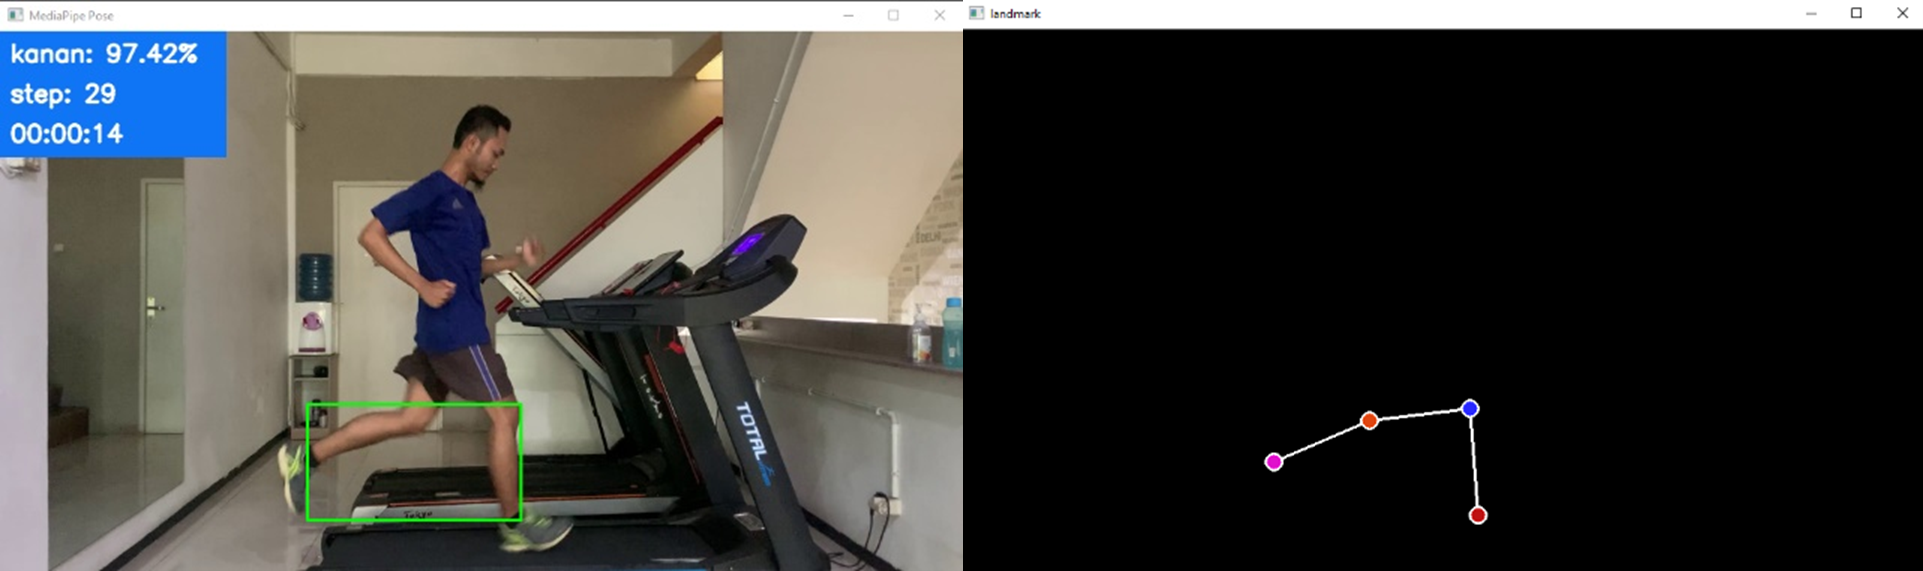
\includegraphics[width=0.4\textwidth]{gambar/deteksi pose.png}
  \caption{Deteksi Pose dengan Mediapipe}
  \label{fig:EstimasiPose}
\end{figure}

Fitur dibuat berdasarkan segmentasi pose yang telah ditentukan dan dilakukan estimasi. Semua fitur dipersiapkan sebagai kombinasi dataset yang nantinya akan digunakan pada training. Setelah menentukan fitur yang akan diekstrak, dilakukan ekstrak fitur untuk mendapatkan setiap data yang dibutuhkan dengan setiap percobaan dari kombinasi segmentasi pose. Hasil yang didapat dari ekstrak fitur berupa data set yang nantinya akan dilakukan training untuk model yang diinginkan. Dataset yang digunakan terdiri dari dua kelas dan pelabelan dari hasil deteksi dan estimasi pose, yaitu kaki “kiri” dan “kanan” seperti pada Gambar \ref{fig:DeteksiPose2}. Hasil pelabelan yang dilakukan pada hasil estimasi dan ekstrak fitur ditunjukkan pada Tabel \ref{tab:HasilAnotasi}

\begin{figure} [ht]
  \centering
  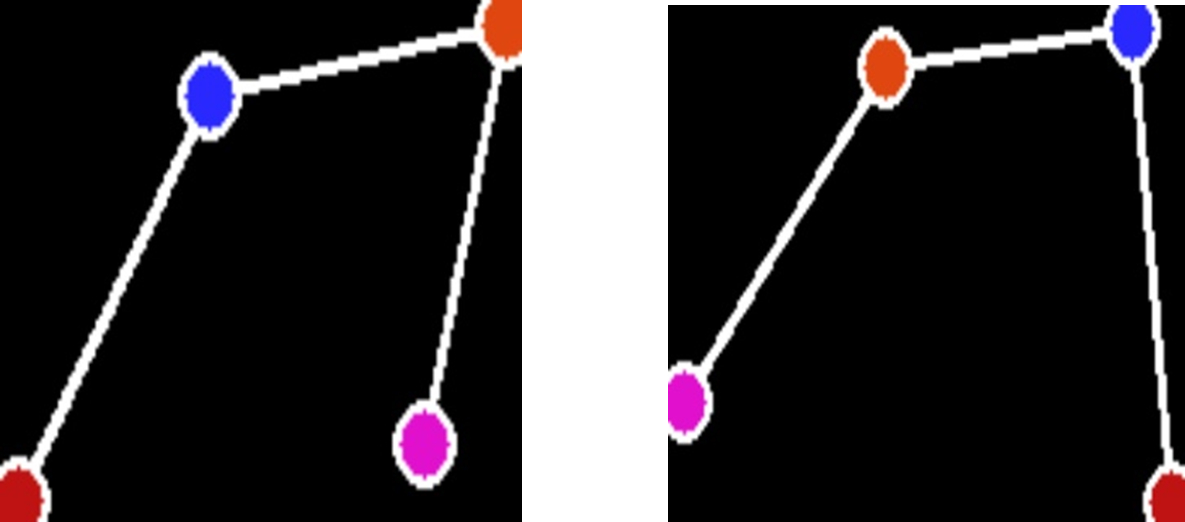
\includegraphics[width=0.4\textwidth]{gambar/deteksi pose2.png}
  \caption{Dataset Pembuatan Model}
  \label{fig:DeteksiPose2}
\end{figure}

\begin{table} [ht]
  \caption{Hasil anotasi pelabelan objek}
  \label{tab:HasilAnotasi}
  \centering
  \begin{tabular}{ll}
    \toprule
    Kelas & Jumlah Anotasi  \\
    \midrule
    Kanan       & 888    \\
    Kiri        & 843    \\
    \textbf{Total}       & \textbf{1.731}        \\
    \bottomrule
  \end{tabular}
\end{table}

\subsection{Klasifikasi Langkah}
\label{subsec:KlasifikasiLangkah}

Fitur yang telah dilakukan ekstraksi maka kemudian dilakukan training untuk memperoleh model deteksi. Model deteksi dari data set akan digunakan untuk melatih model dari sebuah algoritma pada Machine Learning. Dalam melakukan klasifikasi menggunakan Convolutional Neural Networks (CNN). Proses training ini bertujuan agar nantinya komputasi yang dilakukan dalam proses deteksi akan dapat diolah berdasarkan akuisisi data citra menjadi bentuk atau pola pemahaman yang diinginkan. Hasil training akan didapatkan model yang digunakan untuk melakukan klasifikasi atas dataset yang dimiliki yaitu terdapat dua kelas atau label untuk dapat diklasifikasikan menjadi kaki “kiri” dan “kanan”. Klasifikasi dalam menentukan aktivitas yang digunakan pada penelitian ini adalah dapat mengetahu langkah dari seseorang yang berjalan atau berlari seperti pada Gambar \ref{fig:DeteksiModel}.

\begin{figure} [ht]
  \centering
  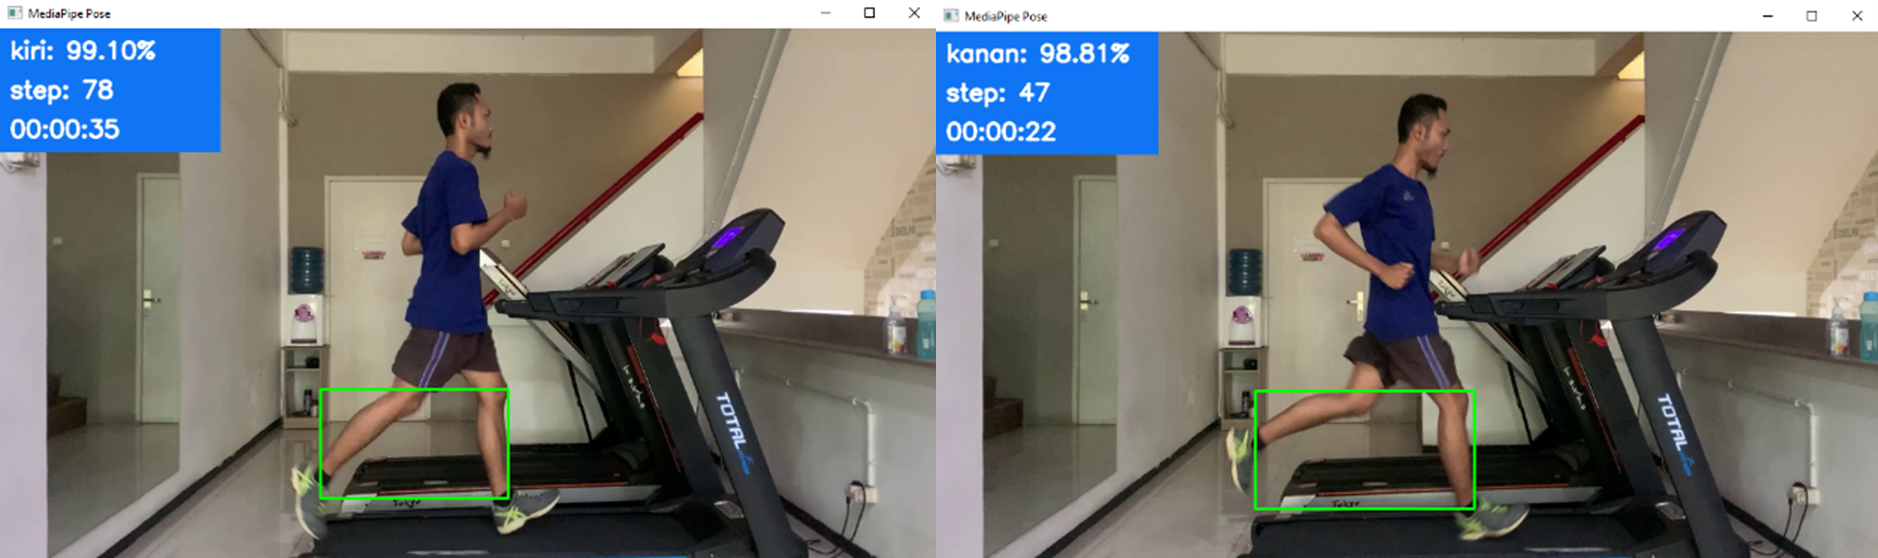
\includegraphics[width=0.4\textwidth]{gambar/deteksi.png}
  \caption{Klasifikasi pada Data Citra}
  \label{fig:DeteksiModel}
\end{figure}



Bentuk hasil klasifikasi yang dibuat adalah mendeteksi pose aktivitas dengan dapat menghitung langkah dan waktu yang ditempuh. Nilai langkah dan waktu yang ditempuh akan digunakan dalam perhitungan selanjutnya. Banyaknya jumlah langkah yang didapat saat hasil deteksi digunakan sebagai nilai variable pertama yang akan digunakan dalam penentuan perhitungan kalori. Langkah dideteksi dan dihitung seberapa banyak langkah yang dilakukan saat proses deteksi. Waktu tempuh saat proses deteksi merupakan nilai variabel kedua yang akan digunakan dalam penentuan perhitungan kalori. Waktu tempuh dimulai saat dideteksi pertama kali nilai langkah yang ditemukan hingga saat akhir langkah tidak ada penambahan kembali yang menandakan proses deteksi telah selesai. Hasil deteksi akan ditampilkan seiring dengan proses deteksi yang dilakukan pada data citra seperti pada Gambar \ref{fig:HasilDeteksi}.

\begin{figure} [ht]
  \centering
  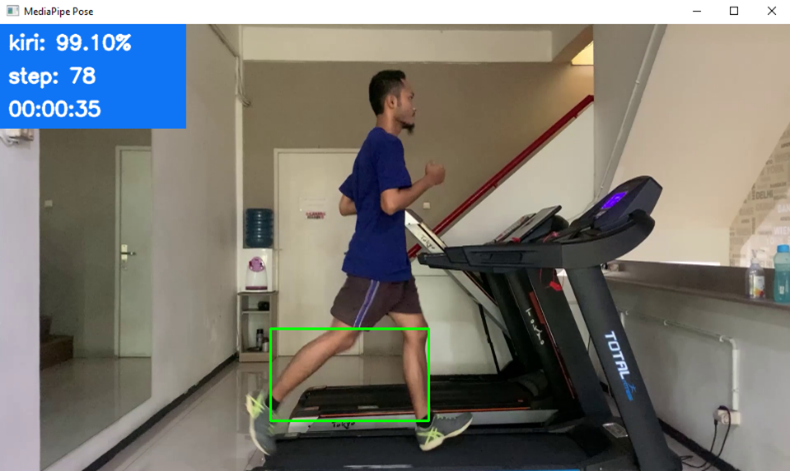
\includegraphics[width=0.4\textwidth]{gambar/hasil deteksi.png}
  \caption{Hasil Deteksi pada Citra}
  \label{fig:HasilDeteksi}
\end{figure}

\subsection{Prediksi Kalori}
\label{subsec:PrediksiKalori}

Prediksi kalori dilakukn dengan dua metode, yaitu menggunakan metode regresi linear dan menggunakan perhitungan rumus EC (Exercise Calories) berdasarkan satuan ukuran MET (Metabolic Equivalent). Kedua metode prediksi ini digunakan sebagai pembanding dalam melakukan analisa terhadap hasil yang didapatkan dari metode prediksi menggunakan metode regresi linear dengan perhitungan rumus. Data yang digunakanan dalam proses prediksi kalori diambil berdasarkan hasil klasifikasi dan hasil deteksi yang telah dilakukan sebelumnya. Hasil deteksi berupa banyaknya langkah dan waktu tempuh digunakan untuk proses prediksi kalori baik dengan metode regresi linear maupun metode perhitungan rumus.

\begin{enumerate}
  \item Regresi Linear
  
  Prediksi kalori dengan regresi linear dilakukan dengan teknik analisis untuk mengidentifikasi relasi antar dua variabel atau lebih. Pada penelitian ini varibel yang digunakan adalah hasil deteksi berupa hasil jumlah deteksi langkah dengan hasil waktu tempuh untuk nantinya akan dicari terkait relasi antara variabel tersebut untuk bisa menentukan hasil yang diinginkan yaitu prediksi kalori. Pengambilan data dilakukan dengan melakukan variasi pada alat treadmill dan didapat data waktu, keepatan dan kalori terbakar untuk dijadikan dataset model regresi. Didapatkan 1045 data sebagai dataset untuk membuat model yang akan dilakukan pengolahan data untuk dapat mendapatkan model yang diinginkan.

  Pengolahan data dilakukan dengan mengubah kecepatan menjadi jarak tempuh berdasarkan data kecepatan dan waktu. Hasil pengolahan data membuat dataset yang digunakan adalah data waktu, jarak tempuh dan kalori terbakar. Model regresi dibuat dengan menggunakan variabel independen berupa waktu dan jarak tempuh, sedangkan variabel dependen berupa kalori terbakar. Hasil proyeksi dari model regresi linear yang dibuat untuk prediksi kalori terbakar ditunjukkan pada Gambar \ref{fig:ModelRegresiKalori}.

  \begin{figure} [ht]
    \centering
    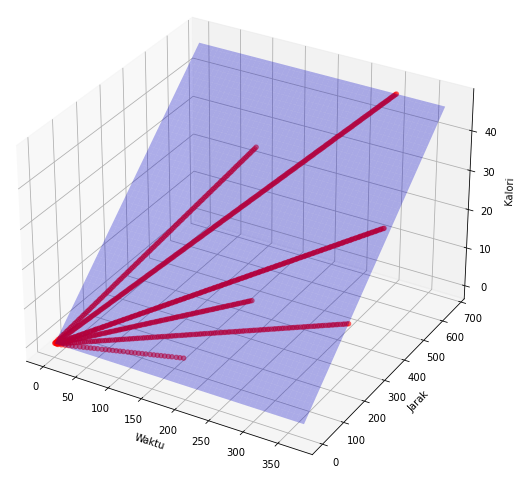
\includegraphics[width=0.4\textwidth]{gambar/model regresi kalori3.png}
    \caption{Model Regresi Linear Prediksi Kalori Terbakar}
    \label{fig:ModelRegresiKalori}
  \end{figure}

  Hasil deteksi berupa banyak langkah dan waktu tempuh diperlukan untuk melakukan pengolahan data banyak langkah menjadi jarak tempuh. Dalam menentukan jarak tempuh diperlukan untuk dapat melakukan prediksi panjang langkah untuk dikalikan dengan banyak langkah dan menghasilkan jarak tempuh. Prediksi jarak tempuh dilakukan dengan model regresi polinomial dengan dataset yang diolah menjadi data waktu, banyak langkah dan panjang langkah. Model regresi dibuat dengan menggunakan variabel independen berupa waktu dan banyak langkah, sedangkah variabel dependen berupa panjang langkah. Hasil proyeksi dari model regresi polinomial yang dibuat untuk prediksi panjang langkah ditunjukkan pada Gambar \ref{fig:ModelRegresiPanjang}.

  \begin{figure} [ht]
    \centering
    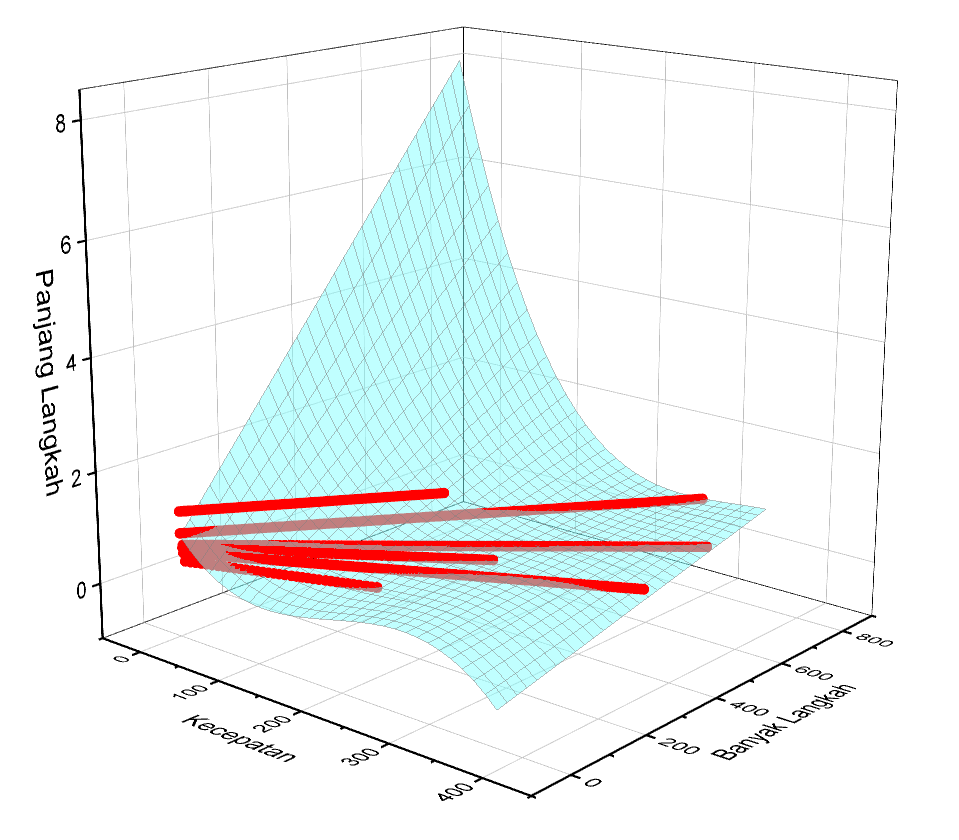
\includegraphics[width=0.4\textwidth]{gambar/model regresi panjang.png}
    \caption{Model Regresi Linear Prediksi Kalori Terbakar}
    \label{fig:ModelRegresiPanjang}
  \end{figure}

  Prediksi kalori dengan regresi dilakukan dengan mengolah hasil deteksi berupa data banyak langkah dan waktu tempuh untuk diprediksi panjang langkah dengan model regresi polinomial prediksi panjang langkah. Kemudian hasil panjang langkah dikali dengan banyak langkah untuk diketahui jarak tempuh. Hasil jarak tempuh dan waktu tempuh diprediksi untuk kalori terbakar dengan model regresi linear prediksi kalori terbakar.

  \item 
  
  Perhitungan Rumus 

  Perhitungan kalori dilakukan dengan mengacu pada nilai satuan ukuran \emph{Metabolic Equivalent} (MET). Satuan MET akan mendapat pengukuran untuk konsumsi oksigen dan pembakaran kalori. Nilai dari satuan MET dapat didefinisikan pada Persamaan \ref{eq:SatuanMET}.

  \begin{equation}
    \label{eq:SatuanMET}
    1 \mathbf{MET} = 3.5 ml O_2  / KG / min
  \end{equation}

  Berdasarkan nilai satuan ukuran MET, didapatkan suatu persamaan untuk menghitung pembakaran kalori yang didefiniskan pada Persamaan \ref{eq:RumusKalori}.

  \begin{equation}
    \label{eq:RumusKalori}
    \mathbf{Cal} = \frac{MET  * 3.5 * BB}{200} * \frac{duration}{60} calories / min
  \end{equation}

  Pada persamaan pembakaran kalori yang akan digunakan untuk melakukan perhitungan pembakaran kalori dari aktivitas yang dilakukan dibutuhkan beberapa nilai variabel untuk mendapatkah hasil total pembakaran kalori, yaitu nilai MET, nilai berat badan (BB), dan nilai waktu tempuh dalam menit.

  Setiap aktivitas memiliki nilai MET yang berbeda-beda dan telah ditentukan oleh peneliti yang telah merangkum banyak aktivitas untuk ditentukan berapa nilai MET yang dihasilkan. Pada aktivitas olahraga yang difokuskan saat ini adalah \emph{jogging} pada treadmill juga memiliki perbedaan nilai MET yang dipengaruhi oleh kecepatan. Data berkaitan dengan pengaruh kecepatan terhadap MET didapatkan yang kemudian dijadikan dataset untuk dilakukan pembuatan model regresi linear prediksi MET. Model regresi dibuat dengan menggunakan variabel independen berupa kecepatan dan variabel dependen berupa MET. Hasil proyeksi dari model regresi linear yang dibuat untuk prediksi MET ditunjukkan pada Gambar \ref{fig:ModelRegresiMET}.

  \begin{figure} [ht]
    \centering
    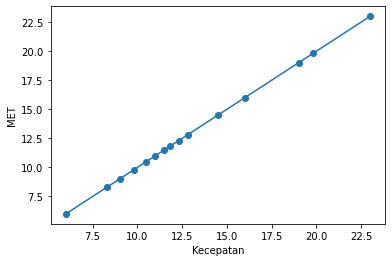
\includegraphics[width=0.4\textwidth]{gambar/model regresi met.png}
    \caption{Model Regresi Linear Prediksi MET}
    \label{fig:ModelRegresiMET}
  \end{figure}
  
  Prediksi kalori dengan perhitungan dilakukan dengan mengolah hasil deteksi berupa data banyak langkah dan waktu tempuh untuk diprediksi panjang langkah. Kemudian hasil panjang langkah dikali dengan banyak langkah untuk diketahui jarak tempuh. Hasil jarak tempuh dan waktu tempuh akan diolah untuk diketahui kecepatan tempuh. Kecepatan tempuh yang didapat dilakukan prediksi untuk MET dengan model regresi linear prediksi MET. Hasil nilai MET digunakan pada perhitungan kalori terbakar dengan data MET, waktu tempuh dan berat badan dengan nilai standar yaitu 70 kg untuk mendapatkan hasil prediksi perhitungan kalori yang terbakar.

\end{enumerate}

